\documentclass[11pt,twocolumn]{article}
\usepackage{subcaption}
\usepackage{fullpage}
\usepackage{pslatex}
\usepackage{tabularx}
\usepackage{booktabs}
\usepackage[table]{xcolor}
\usepackage{graphicx}
\usepackage{amsmath}
\usepackage{listings}
\lstset{basicstyle=\ttfamily, frame=single, language=python, tabsize=4}
\usepackage{tikz}
\usetikzlibrary{arrows.meta, automata, quotes, positioning, babel, shapes.geometric, arrows}

\def\abstract{
	\typeout{Abstract}
	{\bf Abstract} 
} \def\endabstract{\par}

\begin{document}
\title{Model R: Link Weight Prediction with Deep Learning}
\author{
	Yuchen Hou\\
	School of Electrical Engineering and Computer Science \\
	Washington State University, Pullman, WA 99164 \\
	yuchen.hou@wsu.edu
	\and
	Lawrence B. Holder\\
	School of Electrical Engineering and Computer Science \\
	Washington State University, Pullman, WA 99164 \\
	holder@wsu.edu
}
\maketitle

\begin{abstract}
Deep learning has been successful in various domains 
including image recognition, speech recognition and natural language 
processing.
However, the research on its application in graph mining is 
still in an early stage.
Here we present Model R, a neural network model created to provide a deep 
learning approach to the link weight prediction problem.
This model uses a node embedding technique that extracts node embeddings (
knowledge of nodes) from the known links' weights (relations between nodes) and 
uses this knowledge to predict the unknown links' weights.
We demonstrate the power of Model R through experiments and compare it with 
the stochastic block model and its derivatives.
Model R shows that deep learning can be successfully applied to 
link weight prediction and it outperforms stochastic block model and its derivatives by up to 73\% in terms of prediction accuracy.
We analyze the node embeddings to confirm that closeness in embedding space correlates with stronger relationships as measured by the link weight.
We anticipate this new approach will provide effective solutions to more
graph mining tasks.
\end{abstract}

\section{Introduction}
Both academia and industry have seen pervasive adoption of deep learning 
techniques powered by neural network models since the early 2010s,
when they began to outperform other machine learning techniques in various 
application domains, e.g.,
speech recognition \cite{hannun2014deep},
image recognition \cite{simonyan2014very},
natural language processing \cite{yao2013recurrent},
recommendation systems \cite{barkan2016item2vec},
and graph mining \cite{grover2016node2vec}.
These neural net models can not only achieve higher prediction accuracy than 
traditional models,
but also require much less domain knowledge and engineering.

Among those domains,
graph mining is a new and active application area for deep learning.
An important task in graph mining is link prediction \cite{liben2007link} 
\cite{al2006link}, i.e., link existence prediction:
to predict the existence of a link.
A less well-known problem is link weight prediction: to predict the weight of a link.
Link weight prediction is more informative in many scenarios.
For example, when describing the connection of two users in a social network,
a description ``Alice texts Bob 128 times per day" is more informative than
``Alice texts Bob".

We want to create a technique to predict link weights in a graph using a 
neural net model.
The estimator should learn to represent the graph in a meaningful way and learn to predict the target link weights using the representation it learns.

The contribution of this paper is
a first deep learning approach to the link weight prediction problem.
We introduce Model R - the first deep neural network model specifically designed to solve the link weight prediction problem.
We systematically study Model R's node embedding technique and illustrate its uniqueness compared to other embedding techniques.
We also show that Model R significantly outperforms the state of the art non-deep learning approach to the link weight prediction problem - the stochastic block model.

The rest of the paper includes the following sections:
\begin{itemize}
	\item Problem: a description of the link weight prediction problem, including a social network message volume prediction example and a formal definition.
	\item Existing approaches: a review of the state of the art approaches to the link weight prediction problem, including Node Similarity Model, Stochastic Block Model and models derived from Stochastic Block Models.
	\item Deep learning and embeddings: a review of latest deep learning embedding techniques including content based techniques and relation based techniques.
	\item Approach: an introduction to Model R, including its neural network architecture, node embedding technique, deep learning techniques, design parameters and choices.
	\item Experiments: an experimental evaluation of the performance of Model R, with comparison to 4 baseline approaches on 4 datasets.
	\item Node embedding analysis: an analysis of the node embeddings Model R produces to confirm that closeness of nodes in embedding space correlates with strength of node relations.
	\item Conclusion: Model R outperforming Stochastic Block Model shows deep learning can be applied to the link weight prediction problem and achieve better performance than the state of the art non-deep learning approaches.
	\item Future work: a brief discussion of possible future directions of this work.
\end{itemize}

\section{Problem}
We consider the problem of link weight prediction in a weighted directed graph.
We first show an example of the problem,
and then give the problem definition.
An undirected graph can be reduced to a directed graph by converting each weighted undirected link to two directed links with the same weight and opposite directions,
so the prediction for a weighted undirected graph is a special case of the problem we consider.

\subsection{Problem example}
Let us look at an example of link weight prediction, message volume prediction in a social network, shown in Figure \ref{fig:example}.
In this example, there are 3 users in a social network: A, B and C.
Each user can send any amount of text messages to every other user.
We know the number of messages transmitted between A and C, B and C, but not A and B.
We want to predict the number of messages transmitted between A and B.
\begin{figure}[!htb]\centering
	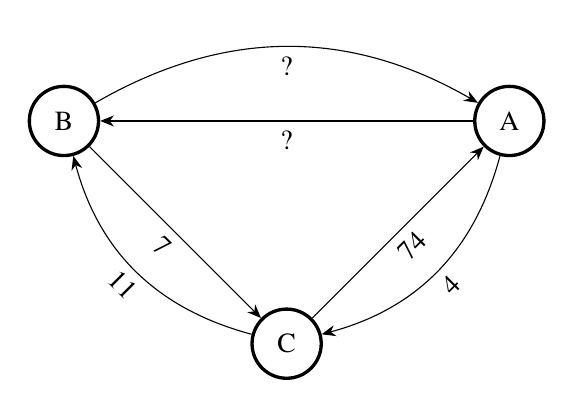
\begin{tikzpicture}[
	node distance = 4cm,
	on grid,
	> = {Stealth[length=5pt,width=4pt]},
	every state/.style = {very thick},
	every edge quotes/.style = {sloped, anchor=north}
	]
	\node[state] (B) {B};
	\node[state] (C) [below right=of B] {C};
	\node[state] (A) [above right=of C] {A};
	\path[->]   
	(A) edge["?"]   (B)
	(B) edge["7"]   (C)
	(C) edge["74"]  (A)
	(B) edge[bend left,"?"]   (A)
	(A) edge[bend left,"4"]   (C)
	(C) edge[bend left,"11"]  (B);
	\end{tikzpicture}
	\caption{
		An example of link weight prediction in a weighted directed graph -
		message volume prediction in a social network.
		}
	\label{fig:example}
\end{figure}

This is a simplified network similar to many real social networks, where every user interacts with other users by posting, sharing, following or liking them.
There can not be any logical approach to derive the unknown message volumes,
as they have randomness.
But there can be statistical approaches to build models to predict them.
The ability to predict these interactions potentially allows us to recommend new connections to users:
if A is predicted/expected to send a large number of messages to B by some model,
and A is not connected to B yet,
we can recommend B as a new connection to A.

\subsection{Problem definition}
Now we define the link weight prediction problem in a weighted directed graph.
\begin{itemize}
	\item Given a weighted directed graph with the node set V and link subset E
	\item Build a model w = f(x, y) where x and y are nodes and w is the weight of link (x, y) that can predict the weight of any link
\end{itemize}
For every possible link (1 out of $ n^2 $, where n is the number of nodes), 
if we know its weight, we know it exists;
if we do not know its weight, we do not know if it exists.
This is a very practical point when we handle streaming graphs:
for any possible link,
we either know it exists and know its weight (if it has been streamed in), or we do not know if the link will ever exist, nor know its weight.

\section{Existing approaches}
In our literature study on previous research in the link weight prediction problem,
we have found some existing approaches, but none use deep learning.
In this section,
we review these existing approaches.

\subsection{Node Similarity Model}
This approach is designed for undirected graphs.
It assumes the weight of a link between two nodes 
is proportional to the similarity of those two nodes.
It employs a linear regression model \cite{zhao2015prediction}:
\begin{align*}
	w_{xy} = k \cdot s_{xy}
\end{align*}
where k is the regression coefficient,
$ w_{xy} $ is the weight of the link between node x and node y,
and $ s_{xy} $ is the similarity of x and y, calculated based on their common neighbors:
\begin{align*}
	s_{xy} = \sum_{z \in N(x) \cap N(y)} F
\end{align*}
where N(x) is the set of neighbors of node x, z is any common neighbor of x and y,
and F is an index factor which has nine different forms, shown in Table \ref{tab:indexes}.
\begin{table*}[!ht]\centering
	\caption{9 different forms of index factor F.}
	\begin{tabularx}{\textwidth}{>{\columncolor{blue!30}}cXXX}  \hline \rowcolor{blue!30}
		& Common Neighbors & Adamic-Adar & Resource Allocation \\ \hline
		Unweighted F &
		\[1\] &
		\[\frac{1}{\log(d_z)}\] &
		\[\frac{1}{d_z}\] \\ \hline
		Weighted F &
		\[w_{xz} + w_{zy}\] &
		\[\frac{w_{xz} + w_{zy}}{\log(1 + s_z)}\] &
		\[\frac{w_{xz} + w_{zy}}{s_z}\] \\ \hline
		Reliable-route Weighted F &
		\[ w_{xz} \cdot w_{zy}\] &
		\[\frac{w_{xz} \cdot w_{zy}}{\log(1 + s_z)}\] &
		\[\frac{w_{xz} \cdot w_{zy}}{s_z}\] \\ \hline
	\end{tabularx}
	\label{tab:indexes}
\end{table*}
In Table \ref{tab:indexes}, $ d_z $ is the degree of node z and $ s_z $ is the strength of node z:
\begin{align*}
s_z = \sum_{u \in N(z)} w_{zu}
\end{align*}
These nine forms represent three groups of measures of 2-hop paths connecting those two nodes:
\begin{itemize}
	\item Unweighted group \cite{adamic2003friends}:
	this group is based on path existence and ignore path weights.
	\item Weighted group \cite{murata2007link}:
	this group is based on path length, i.e., the sum of path weights.
	\item Reliable route weighted group \cite{taha1982operations}:
	this group is based on path reliability, i.e., the product of path weights.
\end{itemize}
And each group contains three forms:
\begin{itemize}
	\item Common Neighbors: this form is based on paths and ignores node degrees.
	\item Adamic-Adar: this form is similar to Common Neighbors,
	but depresses the contribution of nodes with high degrees or high strengths.
	\item Resource Allocation: this form is similar to Adamic-Adar,
	but depresses more than Adamic-Adar does.
\end{itemize}

\subsection{SBM (Stochastic Block Model)}
This approach is designed for unweighted graphs and uses only link existence information \cite{holland1983stochastic}.
The main idea is to partition nodes into L groups and connect groups with bundles.
In this way, the graph has a 2-level structure:
\begin{itemize}
	\item Lower level: each group consists of nodes which were topologically similar in the original graph
	\item Upper level: groups are connected by bundles
	to represent the original graph
\end{itemize}
Given a graph with adjacency matrix A, the SBM has the following parameters:
\begin{itemize}
	\item A: link existence matrix, where $ A_{ij} \in \{0, 1\} $
	\item z: the group vector,
	where $ z_i \in \{ 1 ... L \} $ is the group label of node i
	\item $ \theta $: the bundle existence probability matrix,
	where $ \theta_{z_i z_j} $ is the existence probability of bundle ($z_i, z_j$)
\end{itemize}
So the existence of link (i, j) $ A_{ij} $ is a binary random variable following the Bernoulli distribution:
\begin{align*}
	A_{ij} \sim B(1, \theta_{z_i z_j})
\end{align*}
The SBM fits parameters z and $ \theta $
to maximize the probability of observation A:
\begin{align*}
	P(A|z, \theta) 
	= \prod_{ij} \theta_{z_i z_j}^{A_{ij}}(1-\theta_{z_i z_j})^{1-A_{ij}}
\end{align*}
We rewrite the log likelihood of observation A as an exponential family:
\begin{align*}
	\log(P(A|z, \theta))
	= \sum_{ij} (
	T(A_{ij}) \eta(\theta_{z_i z_j})
	)
\end{align*}
where
\begin{align*}
	T(A_{ij}) = (A_{ij}, 1)
\end{align*}
is the vector-valued function of sufficient statistics of the Bernoulli random variable and
\begin{align*}
\eta(\theta) = ( \log(\frac{\theta}{1-\theta}), \log(1-\theta) )
\end{align*}
is the vector-valued function of natural parameters of the Bernoulli random variable.

\subsection{pWSBM (pure Weighted Stochastic Block Model)}
The pWSBM is designed for weighted graphs and uses only link weight information \cite{aicher2014learning}.
So it differs from SBM in a few ways described below.
Here we choose model link weight with normal distribution.
Adjacency matrix A becomes the link weight matrix where the weight of link (i, j)  $ A_{ij} $ is a real random variable following the normal distribution:
\begin{align*}
A_{ij} \sim N(\mu_{z_i z_j}, \sigma_{z_i z_j}^2)
\end{align*}
$ \theta_{z_i z_j} $ becomes the weight distribution parameter of bundle ($z_i, z_j$):
\begin{align*}
	\theta_{z_i z_j} = (\mu_{z_i z_j}, \sigma_{z_i z_j}^2)
\end{align*}
$ T(A_{ij}) $ becomes the vector-valued function of sufficient statistics of the normal random variable:
\begin{align*}
	T(A_{ij}) = (A_{ij}, A_{ij}^2, 1)
\end{align*}
$ \eta(\theta) $ becomes the vector-valued function of natural parameters of the normal random variable:
\begin{align*}
	\eta(\theta)
	&= (\frac{\mu}{\sigma^2}, -\frac{1}{2\sigma^2}, -\frac{\mu^2}{2\sigma^2})
\end{align*}
The pWSBM fits parameter z and $ \theta $
to maximize the log likelihood of observation A:
\begin{align*}
\log(P(A|z, \theta))
= \sum_{ij} (
A_{ij} \frac{\mu_{z_i z_j}}{\sigma_{z_i z_j}^2}
- A_{ij}^2 \frac{1}{2\sigma_{z_i z_j}^2}
- \frac{\mu_{z_i z_j}^2}{\sigma_{z_i z_j}^2}
)
\end{align*}

\subsection{bWSBM (balanced Weighted Stochastic Block Model)}
The bWSBM is a hybrid of SBM and pWSBM
and uses both link existence information and link weight information \cite{aicher2014learning}.
The hybrid log likelihood becomes:
\begin{align*}
&\log(P(A|z, \theta))\\
=& \alpha \sum_{ij \in E} (T_e(A_{ij}) \eta_e(\theta_{z_i z_j}))\\
& + (1 - \alpha) \sum_{ij \in W} (T_w(A_{ij}) \eta_w(\theta_{z_i z_j}))
\end{align*}
where pair $ (T_e, \eta_e) $ denotes the family of link existence distributions in SBM
and pair $ (T_w, \eta_w) $ denotes the family of the link weight distributions in pWSBM.
and $ \alpha \in [0, 1]$ is a tuning parameter that determines their relative importance,
E is the set of observed interactions,
and W is the set of weighted edges.
In the following, we use $ \alpha = 0.5 $ following the practice in \cite{aicher2014learning}.

\subsection{DCWBM (Degree Corrected Weighted Stochastic Block Model)}
The DCWBM is designed to incorporate node degree
by replacing pair $ (T_e, \eta_e) $ in the bWSBM with:
\begin{align*}
	T_e(A_{ij}) &= (A_{ij}, -d_id_j)\\
	\eta_e(\theta) &= (\log\theta, \theta)
\end{align*}
where $ d_i $ is the degree of node i \cite{aicher2014learning}.

\section{Deep Learning and Embeddings}
As deep learning techniques become more powerful and standardized,
a key process of a domain-specific deep learning application
is converting entities to points in an embedding space, or equivalently,
mapping entities to vectors in a vector space,
because a neural net needs vectors as inputs.
These vectors are called embeddings and this process is called embedding.
Embeddings are ubiquitous in deep learning,
appearing in natural language processing (embeddings for words), recommender systems (embeddings for users and items),
graph mining (embeddings for nodes) and other applications.
In this section, we review a few classical embedding techniques and models for images, audio, words, documents, items and nodes.
A common goal of these techniques is to ensure that
similar entities are close to each other in the embedding space.
Observations about this process lead to the deep learning approach to link weight prediction.

\subsection{Entities and representations}
First of all, we summarize how a neural net represents various types of 
entities in different domains with different relations, as shown in 
Table \ref{tab:domains}.
An image in image recognition is represented as
a 2D light amplitude array with dimensions height and width.
An audio/spectrogram in speech recognition is represented as
a 2D sound amplitude array with dimensions time and frequency.
The relation between two images or two audio is not commonly used. 
Words in natural languages, items in recommendation systems, and nodes 
in graphs can be represented by vectors (1D numeric arrays).
The	relations between two words, two items and two nodes are commonly 
used to learn these vectors.
It is clear that representations for all the entities are numeric arrays, 
because neural nets rely on neurons' activations and communications, which 
are both numeric.
\begin{table*}[!ht]\centering
	\caption{
		A summary of various types of entities, their numeric
		representations and inter-entity relations in different domains.
	}
	\begin{tabularx}{\textwidth}{ccXX} \hline \rowcolor{blue!30}
		Domain & Entity & Relations & Representation \\ \hline
		image recognition & image & N/A & 2D light amplitude array[width, height] \\ \hline
		speech recognition & audio/spectrogram  & N/A & 2D sound amplitude array[time, frequency] \\ \hline
		natural language processing & word   & co-occurrences of words in a context & 1D array (i.e., word vector) \\ \hline
		recommendation systems & item   & co-purchases of items in a order & 1D array (i.e., item vector) \\ \hline
		graph mining & node & connections of nods (i.e., links) & 1D array (i.e., node vector) \\ \hline
	\end{tabularx}
	\label{tab:domains}
\end{table*}

\subsection{Mapping entities to vectors}
The word2vec technique in natural language processing is famous for using a neural net to learn to map every 
entity (word in this case) in a vocabulary to a vector without any domain 
knowledge \cite{mikolov2013distributed}.
In a corpus, every word is described/defined only by related words in its 
contexts, by implicit relations between words in word co-occurrences.
Nonetheless, the neural net can learn from word co-occurrences and map words to 
vectors accordingly.
It provides strong evidence that word embedding with the Skip-gram model can extract knowledge about words from the relations between words and represent this knowledge in the word embedding space \cite{mikolov2013linguistic}.
In fact, most subsequent embedding techniques in other domains use the same Skip-gram model, such as
doc2vec \cite{le2014distributed},
item2vec \cite{barkan2016item2vec},
node2vec \cite{grover2016node2vec} and
deep walk \cite{perozzi2014deepwalk}.
All these techniques have achieved high prediction accuracies in their various applications including language modeling, document classification, item rating prediction, and node classification.

\subsection{Content-based embedding techniques}
Techniques in this group extract knowledge about an entity from its content, 
i.e., the input of the neural network is a vector produced from the item's content.
For example, the content can be the pixel values of an image, or the spectrogram of an utterance.
The similarity of these techniques is that the content (the raw input to the neural network) is already a vector.
Therefore, the embedding process is practically a dimensionality reduction process
that converts a high dimensional raw input vector to a low dimensional vector 
containing more abstract knowledge about the input entity.

\subsubsection{Image embedding with auto-encoders}
This is an unsupervised embedding technique commonly used in image recognition  \cite{vincent2008extracting}.
A small auto-encoder neural network model is shown in Figure \ref{fig:audoEncoder}.
\begin{figure}[!ht]	
	\centering
	\newcommand{\layersep}{2cm}
	\newcommand{\vocabularySize}{8}
	\begin{tikzpicture}
	[->, shorten >=1pt,node distance=\layersep]
	\tikzstyle{every pin edge}=[shorten <=1pt]
	\tikzstyle{neuron}=[circle, draw=black, minimum size=16pt, fill=green!30]
	
	\foreach \name / \y in {1,...,\vocabularySize}
	\node(input-\name) [neuron, fill=red!30, pin={[pin edge={<-}]below:}] at (\y, 0) {};	
	\node [below of=input-4, xshift = 0.5cm, yshift = 1cm] {input = the image pixel values};
	
	\foreach \name / \y in {1,...,4}
	\path[xshift=2cm]
	node(hidden1-\name) [neuron] at (\y, 1*\layersep) {};
	
	\foreach \name / \y in {1,...,2}
	\path[xshift=3cm]
	node(hidden2-\name) [neuron] at (\y, 2*\layersep) {};	
	\node [right of=hidden2-2] {embedding layer};
	
	\foreach \name / \y in {1,...,4}
	\path[xshift=2cm]
	node(hidden3-\name) [neuron] at (\y, 3*\layersep) {};
	
	\foreach \name / \y in {1,...,\vocabularySize}
	\node(output-\name) [neuron, fill=blue!30, pin={[pin edge={->}]above:}] at(\y, 4*\layersep) {};
	\node [above of=output-4, xshift = 0.5cm, yshift = -1cm] {output = the image pixel values};
	
	\foreach \source in {1,...,\vocabularySize}
	\foreach \dest in {1,..., 4}
	\path (input-\source) edge (hidden1-\dest);
	
	\foreach \source in {1,...,4}
	\foreach \dest in {1,...,2}
	\path (hidden1-\source) edge (hidden2-\dest);
	
	\foreach \source in {1,...,2}
	\foreach \dest in {1,...,4}
	\path (hidden2-\source) edge (hidden3-\dest);
	
	\foreach \source in {1,...,4}
	\foreach \dest in {1,...,\vocabularySize}
	\path (hidden3-\source) edge (output-\dest);
	\end{tikzpicture}
	\caption{
		A small auto-encoder neural network model with
		1 input layer (red), 3 hidden layers (green), and 1 output layer (blue),	input size 8, embedding size 2.
		Notice that the embedding layer is the innermost hidden layer.
		The hidden layers use rectified linear units.
		The output layer uses linear units.
	}
	\label{fig:audoEncoder}
\end{figure}
The model is a feed-forward neural network.
The output layer and the input layer have the same size.
The hidden layers closer to the input or output layers have larger sizes.
This technique is unique because during training, the input activation and the expected output activation are always the same vector of pixel values of the image.
From the input layer to the embedding layer, the layer size decreases, compressing the information.
It can effectively reduce a high dimensional vector (the activation of a large number of input units with raw pixel values)
to a low dimensional vector (the activations of a small number of hidden units with abstracted meanings)
\cite{hinton2006reducing}.
This technique applies to not only images for image recognition, but also audio spectrogram for speech recognition \cite{feng2014speech} and words for natural language processing \cite{liou2014autoencoder}.

\subsubsection{Audio embedding with convolutional neural network}
This is a supervised deep learning technique commonly used in speech recognition \cite{abdel2014convolutional}.
A small convolutional neural network model is shown in Figure \ref{fig:cnn}.
\begin{figure}[!ht]
	\centering
	\newcommand{\layersep}{1cm}
	\begin{tikzpicture}
	[->, shorten >=1pt,node distance=\layersep]
	\tikzstyle{every pin edge}=[shorten <=1pt]
	\tikzstyle{layer} = [rectangle, text centered, draw=black, fill=green!30]
	
	\node (input) [layer, fill=red!30, pin={[pin edge={<-}]below:}] {direct activation layer};
	\node [below of=input] {input = the audio spectrogram};
	
	\node (hidden1) [layer, above of=input] {convolutional layer};
	\node (hidden2) [layer, above of=hidden1] {pooling layer};
	\node (hidden3) [layer, above of=hidden2] {convolutional layer};
	\node (hidden4) [layer, above of=hidden3] {pooling layer};
	\node (hidden5) [layer, above of=hidden4] {fully connected layer};
	\node [right of=hidden5, xshift = 3cm] {embedding layer};
	
	\node (output) [layer, fill=blue!30, above of=hidden5, pin={[pin edge={->}]above:}] {fully connected layer};
	\node [above of=output] {output = the target label};
	
	\path (input) edge (hidden1);
	\path (hidden1) edge (hidden2);
	\path (hidden2) edge (hidden3);
	\path (hidden3) edge (hidden4);
	\path (hidden4) edge (hidden5);
	\path (hidden5) edge (output);
	
	\end{tikzpicture}
	\caption{
		A small convolutional neural network model with
		1 input layer (red), 5 hidden layers (green), and 1 output layer (blue).
		Notice that the embedding layer is the last hidden layer.
		The hidden layers use rectified linear units.
		The output layer uses softmax units.
		Only layers and the connections between layers are shown, while the units in each layer and the connections between units are not shown.
	}
	\label{fig:cnn}
\end{figure}
The model is a feed-forward neural network.
The input activation is the vector of pixel values of the audio spectrogram.
The output layer uses softmax units to predict the target label,
such as the genre of a song \cite{van2013deep} or the word of an utterance \cite{abdel2014convolutional}.
From the input layer upward,
each convolutional and pooling layer combo extracts more abstract information
than the previous layer.
Eventually, the neural network converts the raw input data to an embedding
at the fully connected layer and uses it to predict the target label.
Most of the studies on convolutional neural networks focus on accurately
predicting the target attributes,
and the concept of entity embedding is under-explored.
This technique applies to not only audio spectrogram for speech recognition, but also images for image recognition \cite{krizhevsky2012imagenet},
letter trigram for natural language processing \cite{collobert2008unified}
and items for recommender systems \cite{elkahky2015multi}.

\subsection{Relation-based embedding techniques}
Techniques in this group extract knowledge about an entity from its relations 
with other entities, such as words, users, items, and nodes.
The input of the neural network is the one-hot encoding vector of an entity.
An example of this encoding is shown in Table \ref{tab:one-hot}.
\begin{table}[!ht]\centering
	\caption{One hot encoding example for a dictionary of words.}
	\begin{tabular}{cc} \hline \rowcolor{blue!30}
		Word & One-hot encoding \\ \hline
		$ w_1 $ & [1, 0, 0, 0, ... 0]       \\ \hline
		$ w_2 $ & [0, 1, 0, 0, ... 0]       \\ \hline
		$ w_3 $ & [0, 0, 1, 0, ... 0]       \\ \hline
		$ w_4 $ & [0, 0, 0, 1, ... 0]       \\ \hline
		... & ...       \\ \hline
	\end{tabular}
	\label{tab:one-hot}
\end{table}
The similarity of these techniques is that each entity does not contain any
information about itself and therefore its one-hot encoding vector is also
a meaningless vector.
In other words, each entity is only defined by its relations with other entities.
Therefore, in the embedding process, the neural network gradually
forms an understanding of the meaning of all entities by observing the relations
between all entities.

\subsubsection{Word embedding with skip-gram model}
This is an unsupervised embedding technique commonly used in natural language processing \cite{mikolov2013linguistic}.
A small skip-gram neural network model is shown in Figure \ref{fig:skipGram}.
\begin{figure}[!ht]
	\centering
	\newcommand{\layersep}{2cm}
	\newcommand{\vocabularySize}{4}
	\newcommand{\embeddingSize}{2}
	\begin{tikzpicture}
	[->, shorten >=1pt,node distance=\layersep]
	\tikzstyle{every pin edge}=[shorten <=1pt]
	\tikzstyle{neuron}=[circle, draw=black, minimum size=16pt, fill=green!30]
	
	\foreach \name / \y in {1,...,\vocabularySize}
	\node[neuron, fill=red!30, pin={[pin edge={<-}]below:}] (input-\name) at (\y, 0) {};
	\node [below of=input-3, yshift = 1cm] {input = word's one-hot encoding};
	
	\foreach \name / \y in {1,...,\embeddingSize}
	\path[xshift=1cm]
	node[neuron] (hidden-\name) at (\y, 1*\layersep) {};
	\node [right of=hidden-2] {embedding layer};
	
	\foreach \name / \y in {1,...,\vocabularySize}
	\node[neuron, fill=blue!30, pin={[pin edge={->}]above:}] (output-\name) at (\y, 2*\layersep) {};
	\node [above of=output-3, yshift = -1cm] {output = context-word probability distribution};
	
	\foreach \source in {1,...,\vocabularySize}
	\foreach \dest in {1,...,\embeddingSize}
	\path (input-\source) edge (hidden-\dest);
	
	\foreach \source in {1,...,\embeddingSize}
	\foreach \dest in {1,...,\vocabularySize}
	\path (hidden-\source) edge (output-\dest);
	
	\end{tikzpicture}
	\caption{
		A small skip-gram neural network model with
		1 input layer (red), 1 hidden layer (green), and 1 output layer (blue),
		vocabulary size 4 and embedding size 2.
		Notice that the embedding layer is the hidden layer.
		The hidden layer uses linear units.
		The output layer uses softmax units.
	}
	\label{fig:skipGram}
\end{figure}
The model is a feed-forward neural network.
The definition of context is the set of words close to the given word.
For example, given the natural language vocabulary \{the, quick, brown, fox, jumps, over, lazy, dog\}, the sentence ``the quick brown fox jumps over the lazy dog", a context radius of 2, and the word ``fox", we have the context of fox \{quick, brown, jumps, over\}.
A natural language corpus has many sentences,
therefore, from these sentences we can produce a dataset where each example is a (word, context-word) pair,
as shown in Table \ref{tab:words}.
\begin{table}[!ht]
	\centering
	\caption{The words dataset for a natural language corpus.}
	\begin{tabular}{cc} \hline \rowcolor{blue!30}
		Input = word & Output = context-word \\ \hline
		... & ...       \\ \hline
		brown & fox \\ \hline
		brown & jumps \\ \hline
		fox & quick \\ \hline
		fox & brown \\ \hline
		fox & jumps \\ \hline
		fox & over \\ \hline
		jumps & brown \\ \hline
		jumps & fox \\ \hline
		... & ...       \\ \hline
	\end{tabular}
	\label{tab:words}
\end{table}
Given a word fox, its context word is a random variable with a probability distribution:
\[P(context\_word = x | given\_word = fox)\]
where
\[x \in vocabulary\]
and the context-word probability distribution sums to 1 over the vocabulary:
\begin{align*}
	&\sum_{x \in vocabulary}P(context\_word = x | given\_word = fox)\\
	&= 1\\
\end{align*}
During each training step, one training example - a (word, context-word) pair - is used.
The input layer is activated by the one-hot encoding of the given word.
The output layer is expected to predict the one-hot encoding of the context-word.
However, as each word can have many possible context-words, there is always a difference between the expected output and the actual output.
After substantial training, a skip-gram neural network model will eventually output the context-word probability distribution.
The embeddings for all words are technically the weights in the embedding layer.
For any natural language corpus and any two words X and Y in this corpus, we have the following equivalent statements:
\begin{itemize}
	\item X and Y have similar meanings
	\item X and Y have similar context-word probability distributions
	\item X and Y have similar embeddings
\end{itemize}
The final outcome is similar words have similar embeddings.
Acquiring these embeddings is often the first step in many natural language processing tasks such as paraphrasing detection \cite{socher2012deep}, constituency parsing \cite{socher2013parsing},
sentiment analysis \cite{socher2013recursive}, and
information retrieval \cite{shen2014latent}.

\subsubsection{Item embedding with skip-gram model}
This is an embedding technique similar to word embedding, commonly used in recommender systems \cite{barkan2016item2vec}.
This technique reduces the item embedding problem to the word embedding problem and then applies the word embedding technique.
For example, given a purchase order \{monitor, keyboard, mouse, printer, scanner\},
we have the context of mouse \{monitor, keyboard, printer, scanner\}.
An e-commerce platform has many purchase orders, which can produce a dataset where each example is an (item, context-item) pair as shown in Table \ref{tab:items}.
\begin{table}[!ht]
	\centering
	\caption{The items dataset for a collection of orders.}
	\begin{tabular}{cc} \hline \rowcolor{blue!30}
		Input = item & Output = context-item \\ \hline
		... & ...       \\ \hline
		keyboard & mouse \\ \hline
		keyboard & printer \\ \hline
		mouse & monitor \\ \hline
		mouse & keyboard \\ \hline
		mouse & printer \\ \hline
		mouse & scanner \\ \hline
		printer & keyboard \\ \hline
		printer & mouse \\ \hline
		... & ...       \\ \hline
	\end{tabular}
	\label{tab:items}
\end{table}
By reducing purchase orders to natural language sentences and items to words,
this technique reduces the item embedding problem to the word embedding problem.
Applying the word embedding technique will produce the desired item embeddings.
The final outcome is similar items have similar embeddings.

\subsubsection{Node embedding with skip-gram model}
This is an embedding technique similar to item embedding, commonly used in
graph mining \cite{perozzi2014deepwalk} \cite{grover2016node2vec}.
This technique reduces the node embedding problem to the word embedding problem and then applies the word embedding technique.
For example, given a walk in a social network of users \{John, Mary, James, Alice, Bob\}, we have the context of James \{John, Mary, Alice, Bob\}.
A graph has many walks, which can produce a dataset where each example is a (node, context-node) pair.
By reducing walks to natural language sentences and nodes to words,
this technique reduces the node embedding problem to the word embedding problem.
The final outcome is similar nodes have similar embeddings.

\subsection{The weakness of skip-gram model in node embedding}
The relation between nodes is quite different from that between words:
\begin{itemize}
	\item The weight of a link from one node to another specifically tells us
	how strong one node connects to the other;
	this type of relation has regular and explicit form:
	entity - relation - entity.
	\item On the other hand, the co-occurrences of words 
	(e.g., in the context ``The quick brown fox jumps over the lazy dog")
	implicitly tell us these words are related
	but do not tell us any specific relations
	(e.g., Are ``quick" and ``brown" related? What is the relation between ``fox" and ``jumps"? Is ``over" a relation or entity?).
\end{itemize}
Natural languages do not have the notion that
all information can be described as entities and their relations, as in graphs.
For a neural net, 
words can simply show up in sequences from day-to-day conversations,
in many flexible and unpredictable ways, with little structure or regularity.
Therefore, the skip-gram model, designed to handle natural languages,
can not take advantage of highly structured data in graphs.
This suggests that a neural net, if correctly designed to handle graphs,
should be able to learn a node-to-vector mapping supervised by the link weight,
in a more specific, direct and simply way than it learns word-to-vector 
mappings supervised by word co-occurrences.

\section{Approach}
Following the above observations,
we build an estimator with a neural net model using a node pair as its input
and the weight of the link connecting the nodes as its output.
Given a weighted graph, from its adjacency list we can produce a dataset where each example is a (source node, destination node, link weight) triplet.
For example, given a social network where nodes are users and link weights are numbers of messages users send to other users, we have its adjacency list dataset as shown in Table \ref{tab:link-list-dataset}.
\begin{table}[!ht]
	\centering
	\caption{The adjacency list dataset for a social network.}
	\begin{tabular}{cc}  \hline \rowcolor{blue!30}
		Input = (source, destination) & Output = weight \\ \hline
		...                        & ... \\ \hline
		(Mary, John) & 8645 \\ \hline
		(John, Mary) & 9346 \\ \hline
		(John, Alice) & 2357 \\ \hline
		(John, Bob) & 9753 \\ \hline
		(Alic, Bob) & 1238 \\ \hline
		...                        & ... \\ \hline
	\end{tabular}
	\label{tab:link-list-dataset}
\end{table}

\subsection{Model R}
We design the model in the estimator as a fully connected neural network model which we call Model R (R as in relation), shown in Figure \ref{fig:model-r}.
We have considered a convolutional neural net as an alternative,
but we decided it would not be a good fit for this application.
The reason is that these node vectors do not have any spacial property
for a convolutional neural network to take advantage of,
compared to the 2D array of an image where the spacial location of each pixel
has significant meaning (e.g., relative distances of pixels).
These node vectors do not have any of the invariance properties of an image either,
such as translation invariance, rotation invariance,
size invariance and illumination invariance.
In this section, we describe the architecture of Model R and the node embedding technique based on this model.
\begin{figure*}[!htb]
	\centering
	\newcommand{\layersep}{1cm}
	\begin{tikzpicture}
	[->, shorten >=1pt,node distance=\layersep]
	\tikzstyle{every pin edge}=[shorten <=1pt]
	\tikzstyle{layer} = [rectangle, text centered, draw=black, fill=green!30]
	
	\node (input1) [layer, fill=red!30, pin={[pin edge={<-}]below:}] {direct activation layer};
	\node [below of=input1, xshift = -2cm] {input = (source node's one-hot encoding,};
	\node (input2) [layer, fill=red!30, pin={[pin edge={<-}]below:}, xshift = 4cm] {direct activation layer};
	\node [below of=input2, xshift = 2cm] {destination node's one-hot encoding)};
	
	\node (hidden11) [layer, above of=input1] {fully connected layer};
	\node [left of=hidden11, xshift = -3cm] {embedding layer};
	\node (hidden12) [layer, above of=input2] {fully connected layer};
	\node [right of=hidden12, xshift = 3cm] {embedding layer};
	
	\node (hidden2) [layer, above of=hidden1, xshift=2cm] {fully connected layer};
	\node (hidden3) [layer, above of=hidden2] {fully connected layer};
	
	\node (output) [layer, fill=blue!30, above of=hidden3, pin={[pin edge={->}]above:}] {fully connected layer};
	\node [above of=output] {output = link weight};
	
	\path (input1) edge (hidden11);
	\path (input2) edge (hidden12);
	\path (hidden11) edge (hidden2);
	\path (hidden12) edge (hidden2);
	\path (hidden2) edge (hidden3);
	\path (hidden3) edge (output);
	
	\end{tikzpicture}
	\caption{
		A simplified version of Model R with 1 input layer (red), 3 hidden layers (green), and 1 output layer (blue).
		Notice that the embedding layer is the first hidden layer.
		The embedding layer and the input layer each has two channels: one channel for the source node and one channel for the destination node.
		The embedding layer uses linear units
		while other hidden layers use rectified linear units.
		The output layer uses linear units.
		Only layers and their connections are shown,
		while the units in each layer and their connections are not shown.
	}
	\label{fig:model-r}
\end{figure*}
The model contains the following layers:
\begin{itemize}
	\item An input layer directly activated by the one-hot encodings of a (source node, destination node) pair.
	\item A hidden embedding layer of linear units.
	This layer maps each node from its one-hot encoding to the corresponding node vector.
	\item Multiple fully connected hidden layers of rectified linear units
	(only two layers are shown in the figure).
	These units employ the rectifier ($ f(x) = \max (0, x) $)
	as their activation function.
	These layers learn to extract more and more abstract weight-relevant 
	information.
	\item An output layer with a linear regression unit.
	This unit employs linear regression ($ f(x) = kx $) as its activation function.
	It learns to predict the link weight as a real number
	using abstracted weight-relevant information.
\end{itemize}

\subsection{Model R node embedding technique}
The Model R based node embedding technique is different from the skip-gram based techniques.
One advantage of the Model R based node embedding technique is that it takes advantage of the highly organized, regular and repeated structure in the relational dataset representing a graph, i.e., a source node connects to a destination node through one and only one weighted link.
The skip-gram model does not exploit this structure in natural language processing because this structure does not exist.
Link weights provide the information about nodes.
We fully take this property into account and design this model to learn 
complex and unobservable node information (i.e., node vectors) 
supervised by a simple and observable relation between nodes (i.e., link weight).

\subsection{Model R learning techniques}
The estimator uses the above model and a number of popular deep learning 
techniques:
\begin{itemize}
	\item Backpropagation: propagation of the error gradients from output layer 
	back to each earlier layer \cite{rumelhart1988learning}
	\item Stochastic gradient descent: the optimization that minimizes 
	the error (descending against the error gradient in weight space) for a 
	random sample in each gradient descent step \cite{lecun2012efficient}
	\item Mini-batch: the modification to stochastic gradient descent to 
	accelerate and smooth the descent by minimizing the error for a small 
	random batch of samples in each gradient descent step \cite{mairal2010online}
	\item Early stopping: the regularization used to reduce over-fitting during the iterative learning process by stopping the learning when validation error stops decreasing \cite{smale2007learning}
\end{itemize}

\subsection{Model R design parameters and choices}
Now we briefly discuss different options for our design parameters and choices,
and also some justifications for our choices.
\begin{itemize}
	\item The choice of rectifier as the activation function is a relatively easy one.
	Compared to earlier popular activation functions like sigmoid function
	($ f(x) = (1 + \exp(-x))^{-1} $),
	rectifier not only simplifies and accelerates computation,
	but also eliminates vanishing gradient problems,
	and has become the most popular activation function
	for deep neural networks \cite{lecun2015deep}.
	\item The choice of layer size is related to
	the number of examples in the dataset.
	Naturally, the larger the dataset is,
	the more discriminative the model should be,
	and consequently higher degrees of freedom,
	higher dimensions of vectors and larger layer sizes.
	Empirically, we usually set the layer size as a logarithm function of the dataset size:
	\[d = log_2(n)\]
	where d (as in dimension) is the layer size and n is the dataset size.
	\item The choice of number of hidden layers is related to the complexity of the relation between the input and the output of the model.
	As a trivial example, if the input and the output have a linear relation,
	no hidden layer is necessary and the model is simply a linear model.
	If the input and the output have a non-linear relation,
	the more complex the relation is, the more layers are necessary.
	Empirically, we usually set the number of hidden layers to 4,
	as a good compromise of learning speed and prediction accuracy.
\end{itemize}
We naturally assume the most optimum design parameters are dataset dependent.
However, we do not know any theoretical way to calculate the most optimum parameters based on the statistic signatures of a specific dataset.
Therefore, in this work, we evaluate different parameter choices through a few experiments.
We will work on design parameter optimization in our future research.

\section{Experiments} \label{section:experiments}
We evaluate Model R experimentally with SBM, pWSBM, bWSBM and DCWBM as baselines,
and compare their prediction errors on several datasets.
We use the same datasets and experiment process used in a recent study of these baselines \cite{aicher2014learning}.
The results show 
that Model R can achieve much lower prediction error than the baseline models.

\subsection{Datasets}
The experiments use four datasets:
\begin{itemize}
	\item Airport \cite{colizza2007reaction}. Nodes represent the busiest airports in the United States, and each of the directed edges is weighted by the number of passengers traveling from one airport to another.
	\item Collaboration \cite{pan2012world}. Nodes represent nations on Earth, and each of the edges	is weighted by a zed count of academic papers whose author lists include that pair of nations.
	\item Congress \cite{porter2005network}. Nodes represent the committees in the 102nd United States Congress, and each of the edges is weighted by the number of shared members.
	\item Forum \cite{opsahl2009clustering}. Nodes represent users of a student social network at UC Irvine, and each of the directed edges is weighted by the number of messages sent between users.
\end{itemize}
The statistics of these datasets are summarized in Table \ref{tab:datasets}.
\begin{table}[!ht]\centering
	\caption{The statistics of the graph datasets used in experiments.}
	\begin{tabular}{cccc} \hline \rowcolor{blue!30}
		Dataset & Node \# & Link \# & Degree \\ \hline
		Airport & 500 & 5960 & 11.92 \\ \hline
		Collaboration & 226 & 20616 & 91.22 \\ \hline
		Congress & 163 & 26569 & 163 \\ \hline
		Forum  & 1899 & 20291 & 10.68 \\ \hline
	\end{tabular}
	\label{tab:datasets}
\end{table}

\subsection{Experiment process}
We do the same experiment for each dataset.
All the link weights are normalized to the range [-1, 1] after applying a logarithm function.
Each experiment consists of 25 independent trials.
In each trial, we split the dataset randomly into 3 subsets:
\begin{itemize}
	\item 70\% into training set
	\item 10\% into validation set
	\item 20\% into testing set
\end{itemize}
We use mean squared error as the prediction accuracy metric.
For each trial we learn using the training set until error on the validation set increases. We then evaluate the error of the learned model on the testing set.
For each experiment, we report the mean and standard deviation of the errors from 25 trials.

\subsection{Experiment results}
In our experiments,
Model R's error is lower than all other models on all datasets,
as shown in Figure \ref{fig:errors} and Table \ref{tab:errors}.
\begin{figure*}[!ht]\centering
	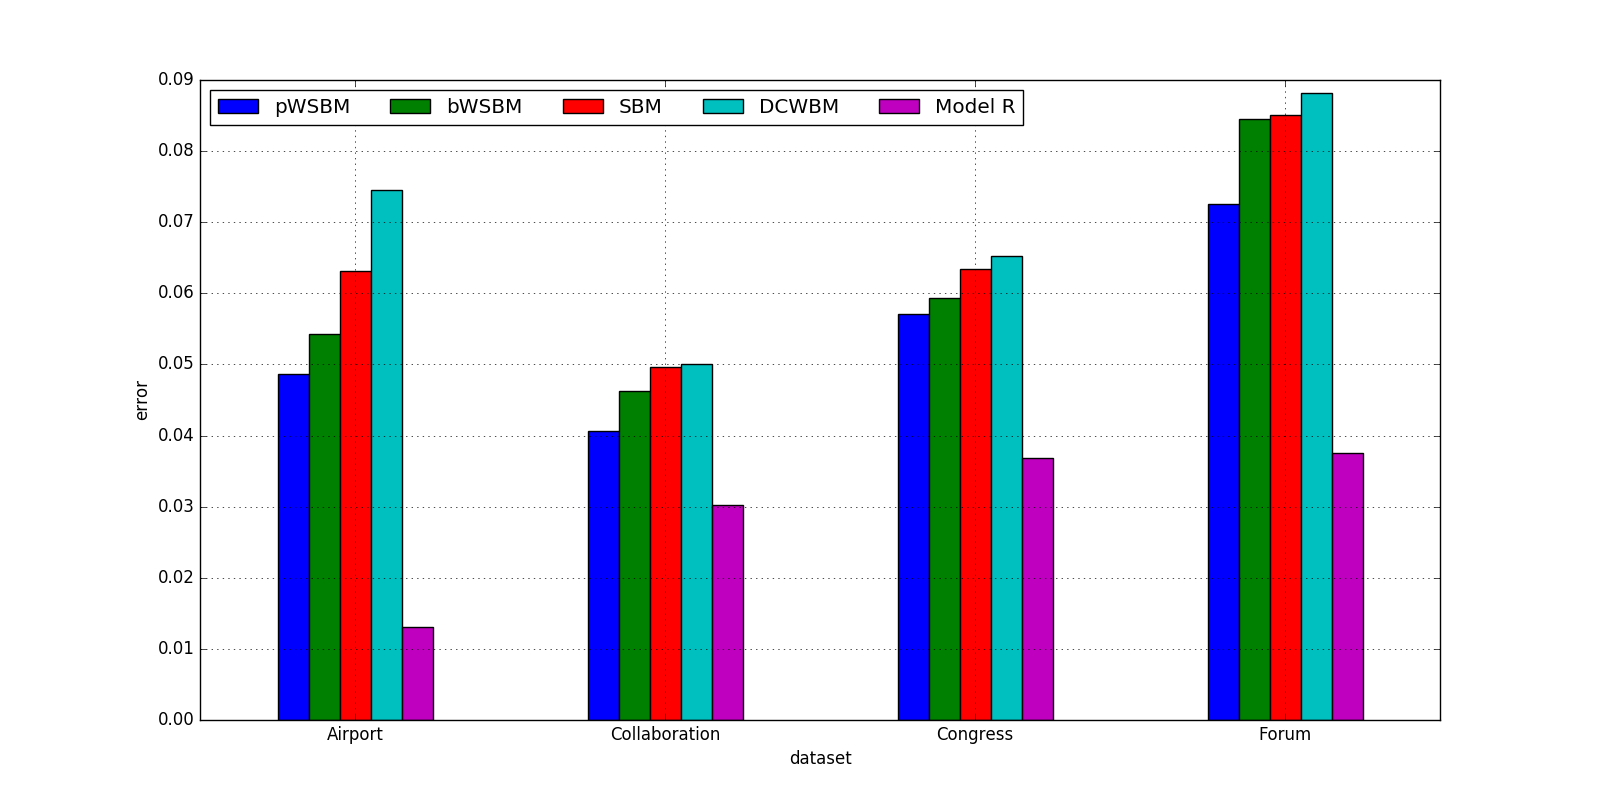
\includegraphics[width=1\textwidth]{link-weight-errors}
	\caption{
		The mean squared errors of 5 models on 4 datasets:
		Model R has lower error than every other model on every dataset.
		Every error value shown here is the mean error for the 25 trials in the experiment.
	}
	\label{fig:errors}
\end{figure*}
\begin{table*}[!htb]\centering
	\caption{
		The mean squared errors with standard deviations of 5 models on 4 datasets.
		Welch's t-test defines its p value as the Student's t-distribution cumulative density function $ p = 2 \int_{-\infty}^{-|t|} f(x) dx $.
	}
	\begin{tabularx}{\textwidth}{|c|X|X|X|X|X|c|c|} \hline \rowcolor{blue!30}
		Dataset & pWSBM & bWSBM & SBM & DCWBM & Model R & Reduction & p \\ \hline
		Airport & 0.0486 $ \pm $ 0.0006 & 0.0543 $ \pm $ 0.0005 & 0.0632 $ \pm $ 0.0008 & 0.0746 $ \pm $ 0.0009 & 0.013 $ \pm $ 0.001 & 73\% & 4.2e-66 \\ \hline
		Collaboration & 0.0407 $ \pm $ 0.0001 & 0.0462 $ \pm $ 0.0001 & 0.0497 $ \pm $ 0.0003 & 0.0500 $ \pm $ 0.0002 & 0.030 $ \pm $ 0.001 & 25\% & 9.1e-44 \\ \hline
		Congress & 0.0571 $ \pm $ 0.0004 & 0.0594 $ \pm $ 0.0004 & 0.0634 $ \pm $ 0.0006 & 0.0653 $ \pm $ 0.0004 & 0.036 $ \pm $ 0.003 & 35\% & 7.1e-35 \\ \hline
		Forum & 0.0726 $ \pm $ 0.0003 & 0.0845 $ \pm $ 0.0003 & 0.0851 $ \pm $ 0.0004 & 0.0882 $ \pm $ 0.0004 & 0.037 $ \pm $ 0.001 & 48\% & 4.2e-68 \\ \hline
	\end{tabularx}
	\label{tab:errors}
\end{table*}
In this section we compare Model R with the baseline models on every dataset.
Given the dataset,
we regard ModelRError (as well as BaselineError) as a random variable
so each trial generates an example of it.
We can do a t-test to justify the significance of the difference between the means of variables ModelRError and BaselineError.
The mean of a variable is not the same as the mean of a sample of the variable.
More specifically, a variable can generate two samples with different sample means,
therefore two samples with different means do not imply the two variables generating them have different means.
For each dataset, we do a t-test for the two variables where the null hypothesis is that the two variables have the same mean:
\begin{align*}
\overline{X_1} == \overline{X_2}
\end{align*}
where $ X_1 $ and $ X_2 $ are ModelRError and BaselineError and
where $ \overline{X} $ is the mean of variable X.
Welch's t-test defines its p value as the Student's t-distribution cumulative density function:
\begin{align*}
p = 2 \int_{-\infty}^{-|t|} f(x) dx
\end{align*}
The smaller p is, the more confidently we can reject the null hypothesis, i.e., accept that:
\begin{align*}
\overline{ModelRError} \neq \overline{BaselineError}
\end{align*}
Typically there is a domain specific threshold for p, e.g., 0.1 or 0.01. If p is smaller than the threshold we reject the null hypothesis.
We calculate the p value and also error reduction from baseline to Model R as:
\begin{align*}
Reduction = \frac{BaselineError - ModelRError}{BaselineError}
\end{align*}
The p value is almost 0 for all datasets and error reduction is significant,
shown in Table \ref{tab:errors}.
Model R has lower error than every other model on every dataset,
reducing error by 25\% to 73\% from the best baseline model - pWSBM.
The number in every parenthesis is the standard deviation of the errors in 25 trials in the last digit. The very low p values strongly indicate the error reduction is significant.
These results show that Model R outperforms pWSBM on all these datasets.

\subsection{Model robustness}
In our experiments, we have not observed any significant (more than 5\%)
prediction error increase or decrease when we change parameters around the values
we typically choose.
Overall, Model R has demonstrated a very high level of model robustness.

\subsection{Reproducibility}
In order to ensure the reproducibility of the experiment,
we specify the implementation details in this section:
\begin{itemize}
	\item Programming language: Python 3
	\item Python implementation: CPython 3.5
	\item Deep learning package: TensorFlow \cite{abadi2016tensorflow}
	\item Operating system: Ubuntu 16.10 64-bit
	\item Memory: 16 GB
	\item Processor: Intel Core i7-4770 CPU @ 3.40GHz
\end{itemize}
The program uses all 8 threads of the processor.
Each experiment takes about one hour to finish,
depending on the dataset and parameters in the learning algorithm.
The program is open-source under MIT license hosted on Github \footnote{https://github.com/yuchenhou/elephant}
so that everyone can use it without any restriction.

\section{Node embedding analysis}
The purpose of this section is to find out what knowledge Model R learns during training.
Our hypothesis is that the knowledge it learns consists of meaningful node embeddings where similar nodes (according to our own (human) semantics associated with the domain's entities) are close to each other in the node embedding space.
We make this hypothesis based on the following observations that Model R and the skip-gram model have similar architecture in their one-hot encoding input layer and linear embedding layer, and that the skip-gram model produces word embeddings where similar words are close to each other in the word embedding space.
Our goal is to verify this hypothesis by analyzing and visualizing the node embeddings produced by Model R in real world datasets from well understood domains to make the results obvious to most readers.

\subsection{Motivation}
Seeing the good performance of Model R, we are interested in this question: what exactly does Model R learn?
Even though Model R outperforms some of the latest link weight prediction techniques by a large margin, the knowledge it learns is not apparent.
We claim that Model R learns knowledge of nodes in the form of node embeddings from the known link weights and uses that knowledge to predict unknown link weights.
This claim is plausible and similar to the claim in the original word2vec paper \cite{mikolov2013linguistic}.
There have been several studies on word2vec focusing on the analysis and visualization of the word embeddings \cite{mikolov2013distributed} \cite{mikolov2013linguistic}.
These studies have provided strong evidences that the word embeddings learned by the skip-gram model represent meaningful knowledge about words.
However, we need to provide evidence that the node embeddings learned by Model R represent knowledge consistent with our understanding of the domain.
If we can have more in-depth study on those node embeddings similar to the studies on word embeddings, we can have a much better understanding of what Model R learns and why it performs well.

\subsection{Methods}
In order to perform node embedding analysis,
the experiment needs additional embedding logging and visualization methods.
The model trains on the datasets and produces node embeddings.
The visualizer reduces the dimension of the embeddings,
attaches domain metadata to the embeddings and produces the final visualization.
The visualization is then analyzed to confirm closeness of semantically-similar nodes.

\subsubsection{Datasets}
In order to verify the knowledge of nodes learned by the model is meaningful (agrees with our domain knowledge), the experiments use real world datasets from two well known domains:
\begin{itemize}
	\item Collaboration \cite{pan2012world}.	
	Nodes represent 226 nations on Earth, and each of the 20616 edges is weighted by the number of academic papers whose author lists include that pair of nations.
	This is the same dataset used in Section \ref{section:experiments} to evaluate the prediction error of Model R.
	\item MovieLens100K \cite{harper2015movielens}.
	This dataset is a recommendation dataset, and also a bipartite graph dataset.
	Nodes represent 1000 users and 1700 movies, and each of the 100000 edges is weighted by the rating score a user has given to a movie.
\end{itemize}
A snippet of MovieLens100K dataset is shown in Table \ref{tab:movielens100k} as an example.
\begin{table}[!ht]
	\centering
	\caption{A snippet of MovieLens100K dataset.}
	\begin{tabular}{ccc}  \hline \rowcolor{blue!30}
		User ID & Item ID & rating \\ \hline
		196 & 272 & 3 \\ \hline
		186 & 302 & 3 \\ \hline
		22 & 377 & 1 \\ \hline
		244 & 51 & 2 \\ \hline
		166 & 346 & 1 \\ \hline
		... & ... & ... \\ \hline
	\end{tabular}
	\label{tab:movielens100k}
\end{table}

\subsubsection{Embeddings}
The embeddings are the vectors the model maps the nodes to, and the vectors these experiments produce for us to visualize and analyze.
Technically, these embeddings are the weights of the embedding layer of Model R shown in Figure \ref{fig:model-r}.

\subsubsection{Metadata}
The metadata provides domain specific information about the datasets necessary to verify the embeddings match our understanding about the specific domain. A snippet of MovieLens100K dataset metadata is shown in Table \ref{tab:movielens100kmeta} as an example.
\begin{table}[!ht]
	\centering
	\caption{A snippet of MovieLens100K dataset metadata.}
	\begin{tabular}{ccc} \hline \rowcolor{blue!30}
		Item ID & Title & Release date \\ \hline
		1 & Toy Story & 01-Jan-1995 \\ \hline
		2 & GoldenEye & 01-Jan-1995 \\ \hline
		3 & Four Rooms & 01-Jan-1995 \\ \hline
		4 & Shanghai Triad & 01-Jan-1995 \\ \hline
		5 & Twelve Monkeys & 01-Jan-1995 \\ \hline
		... & ... & ... \\ \hline
	\end{tabular}
	\label{tab:movielens100kmeta}
\end{table}

\subsubsection{Model training}
The model training process is the same as the previous experiment,
with an extra step to log embedding layer weights.

\subsubsection{Embedding visualization}
The embedding visualization process plays an important role in the final knowledge representation.
This embedding visualization process has the following steps:
\begin{enumerate}
	\item Join the metadata and the embeddings on the node ID to attach the related information provided by the metadata to each node.
	\item Calculate the Euclidean distances between pairs of nodes.
	\item Dimensionality reduction through PCA (principal component analysis) on the embeddings to project these points from the high dimensional embedding space to a 2-dimensional space so that we can visualize them.
	\item Display all embeddings in an image, e.g., Figure \ref{fig:movies} and Figure \ref{fig:countries}.
\end{enumerate}

\subsection{Data analysis and visualization}
The experiment results meet our expectation - nodes more similar to each other (based on their semantics associated with the specific domain) have their corresponding points closer to each other in the embedding space.
The experiment process runs once for each of the two datasets: MovieLens100K and Collaboration.
We present the data analyses on a few well known cases and visualizations on the entire datasets as well.
The analysis for each dataset has the following steps:
\begin{enumerate}
	\item Select a well known reference node in the domain with two similar nodes that are easy to identify.
	\item Sort all nodes with respect to their distances to the reference.
	\item Verify that the distances from the two similar nodes to the reference node are much shorter than that of the median point.
\end{enumerate}
In this section, we perform data analysis on the experiment results for both datasets.

\subsubsection{MovieLens100K}
For this dataset, we select the movie ``Star Wars: The Empire Strikes Back" as the reference movie and the other two movies in the original Star Wars trilogy as the two similar movies, i.e., ``Star Wars: A New Hope" and ``Star Wars: Return of the Jedi".
Notice that we do not need to assume which attributes of a movie have the most influence in users' preferences for movies, because these two movies are similar to the reference movie in many attributes such as genre, actors, screenwriter, distributor and storyline.
The distances of a number of closest movies to the reference movie are shown in Table \ref{tab:movielens100k-distance}.
\begin{table*}[!ht]\centering
	\caption{
		The distances of movies to the reference movie for MovieLens100K dataset.
	}
	\begin{tabular}{ccc} \hline \rowcolor{blue!30}
		Movie & Distance & Similarity \\ \hline
		The Empire Strikes Back (1980) & 0 & self (reference) \\ \hline
		Raiders of the Lost Ark (1981) & 0.012 & most similar \\ \hline
		... & ... & ... \\ \hline
		Star Wars (1977) & 0.047 & more similar \\ \hline
		Return of the Jedi (1983) & 0.063 & more similar \\ \hline
		... & ... & ... \\ \hline
		Children of the Revolution (1996) & 0.256 & median point \\ \hline
		... & ... & ... \\ \hline
		Tomorrow Never Dies (1997) & 0.295 & less similar \\ \hline
		Ayn Rand: A Sense of Life(1997) & 0.296 & less similar \\ \hline
		... & ... & ... \\ \hline
		101 Dalmatians (1996) & 0.335 & least similar \\ \hline
	\end{tabular}
	\label{tab:movielens100k-distance}
\end{table*}
The data indicate that the distances from similar movies to the reference movie are much shorter than that from the median point.
The embeddings of all movies are shown in Figure \ref{fig:movies}.
\begin{figure*}[!ht]\centering
	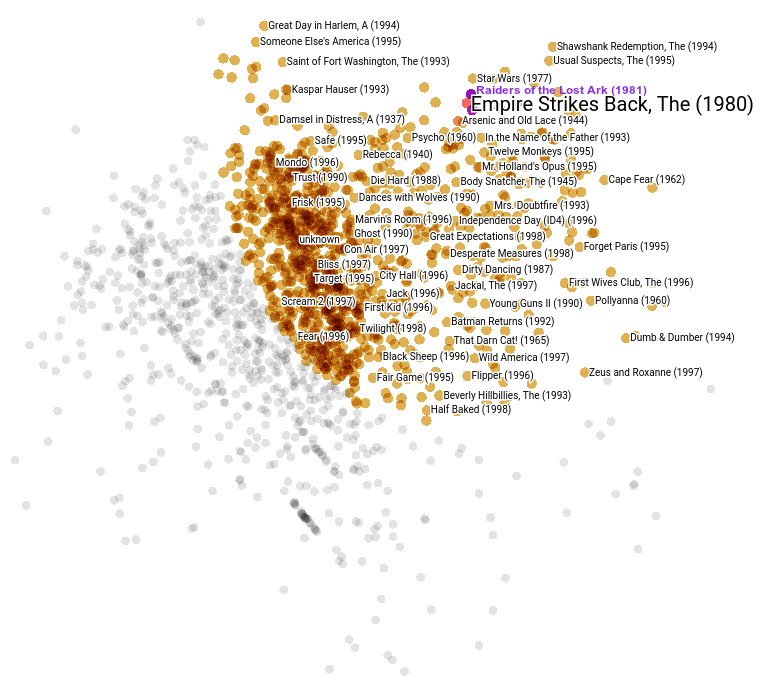
\includegraphics[width=0.8\textwidth]{movies-annotation}
	\caption{
		The embeddings of all movies in MovieLens100K dataset:
		``The Empire Strikes Back" is the reference movie, shown as a red node with bold font name.
		``Raiders of the Lost Ark" is the closest movie to the reference movie, shown as a purple node with purple name.
		A few other close movies are also shown as purple nodes.
		The image does not display names for many movies to avoid overlapping of the text.
		This embedding shows the overall distribution of movies where similar movies are closer to the reference movie.
	}
	\label{fig:movies}
\end{figure*}

\subsubsection{Collaboration}
For this dataset, we select the country United States as the reference country and two other countries with similar economy, education and culture backgrounds as the two similar countries: United Kingdom and Germany.
Notice that we assume economy, education and culture background have the most influence in international collaboration patterns.
The distances of a number of all countries to the reference country are shown in Table \ref{tab:countries-distance}.
\begin{table}[!ht]\centering
	\caption{
		The distances of countries to the reference country for Collaboration dataset.
	}
	\begin{tabular}{ccc} \hline \rowcolor{blue!30}
		Country & Distance & Similarity \\ \hline
		United States & 0 & self (reference) \\ \hline
		China & 0.216 & most similar \\ \hline
		... & ... & ... \\ \hline
		United Kingdom & 0.411 & more similar \\ \hline
		Germany & 0.483 & more similar \\ \hline
		... & ... & ... \\ \hline
		Jamaica & 29.531 & median point \\ \hline
		... & ... & ... \\ \hline
		Senegal & 31.018 & less similar \\ \hline
		Peru & 31.259 & less similar \\ \hline
		... & ... & ... \\ \hline
		Zimbabwe & 32.283 & least similar \\ \hline
	\end{tabular}
	\label{tab:countries-distance}
\end{table}
The data indicate that the distances from similar countries to the reference country are much shorter than that from the median point.
The embeddings of all countries are shown in Figure \ref{fig:countries}.
\begin{figure*}[!ht]\centering
	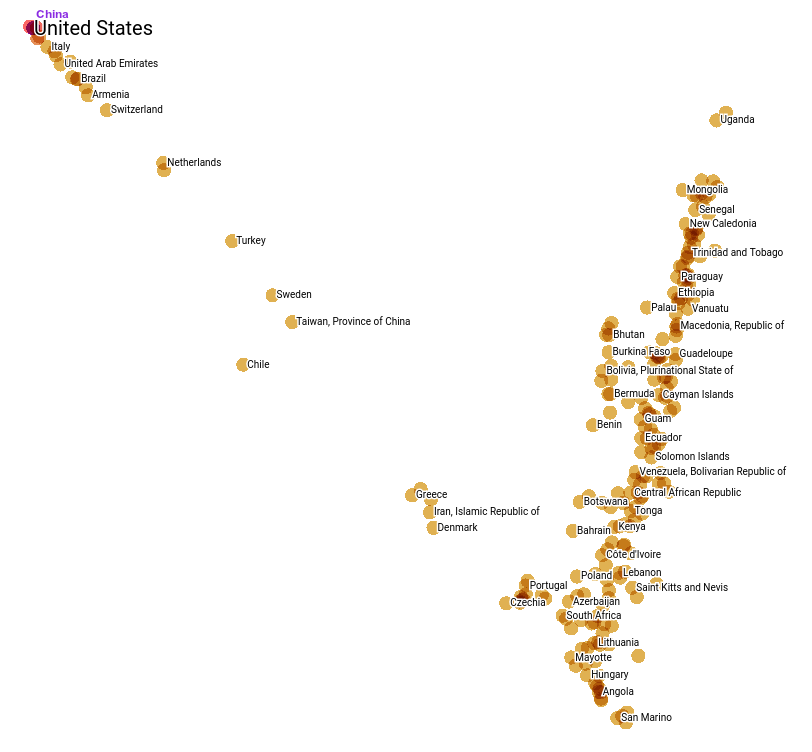
\includegraphics[width=0.8\textwidth]{countries-annotation}
	\caption{
		The embeddings of countries in Collaboration dataset:
		The United States is the reference country, shown as a red node with bold font name.
		China is the closest country to the reference country, shown as a purple node with purple name.
		A few other close countries are also shown as purple nodes.
		The image does not display names for many countries to avoid overlapping of the text.
		This embedding shows the overall distribution of countries where similar countries are closer to the reference country.
	}
	\label{fig:countries}
\end{figure*}

\section{Conclusion}
Model R shows that deep learning can be successfully applied to the link weight prediction problem.
It effectively learns complex and unobservable node information (i.e., node vectors) from simple and observable relations between nodes (i.e., link weights),
and uses that information to predict unknown link weights.
Compared to SBM based approaches, Model R is much more accurate.
A few possible reasons are:
\begin{itemize}
	\item Higher level of discrimination for nodes:
	SBM based approaches do not differentiate nodes within the same group,
	and assume the weights of all links connecting two nodes from two groups
	follow the same distribution.
	Model R does not assume that,
	but gives every node a unique description - the node vector - so that
	it can have a more accurate description for every single node.
	\item Higher level of model flexibility:
	SBM based approaches assume the weight of every link follows
	a normal distribution.
	Model R does not assume that, but takes advantage of high flexibility of
	layers of non-linear neural network units,
	so that it can model very complex weight distributions.
\end{itemize}
Model R learns meaningful node embeddings where similar nodes (based on their semantics associated with the specific domain) are close to each other in the node embedding space.
This work provides direct evidences that deep learning based embedding techniques are effective in two application domains beside natural language processing: recommender systems and graph mining.
We anticipate this new approach will provide effective solutions to more
graph mining tasks.

\section{Future work}
There are a few directions we would like to study in our future work on this model.

\subsection{Node embedding metrics}
An important direction for this work is to identify metrics for evaluating the learned node embeddings.
As embeddings are ubiquitous and valuable in deep learning and the popularity of deep learning is on the rise, we believe an important question is: what are good embeddings?
A direct answer can be: embeddings that match humans' perceptions of the nodes are good embeddings.
But humans' perceptions are, by nature, very complicated and subjective.

As similar nodes should have their embeddings close to each other, a possible metric is the distances of the embeddings of similar nodes.
This is an obvious metric and also the one we tried to use intuitively for this work.
The distance measurement for embeddings is relatively easy but the similarity measurement for nodes is relatively hard.
One possible way to measure similarity is some type of statistics measurement of the behaviors of nodes.
For example, in recommender systems, it is natural to assume two users are very similar if they always give the same ratings to each one of the movies.
The challenge is this metric is not easy to measure if there are few movies rated by both users.
Another possible way to measure similarity is some type of measurement of the distance of their attribute vectors.
For example, the attribute vector of a user can be [age, gender, occupation, location] as exposed by the metadata.
In order for this measure to be useful, we need to know what attributes are the most relevant to users' movie preferences.

Good embeddings should produce good prediction accuracy, despite the type of node targeted for prediction.
This one is very obvious because eventually some other machine learning system should use these embeddings to do valuable predictions.
Therefore, good metrics should have positive correlation with prediction accuracy of the later stages of the deep learning system whose inputs are the embeddings.
This does not require any work with respect to the actual nodes but it is still hard to measure: some embeddings might work well on some models but not on other models, so it is hard to decide which model should be used as the evaluation reference.

\subsection{Complex graphs}
This direction is especially appealing for social network applications.
In particular, we want to handle graphs with node attributes.
Users can have labels like ``nationality", and real attributes like ``age".
One feasible approach is to append one unit for each of these attributes to the node vector.

\subsection{Large dynamic graphs}
A social network can have a large volume of links collected continuously by a
distributed system.
A potential approach is to deploy an estimator to each computing node of
the distributed system and analyze a link stream there,
and let these estimators exchange their knowledge periodically.

\section*{Acknowledgements}
This material is based upon work supported by the National Science Foundation under Grant No. 164640.

\bibliographystyle{IEEEtran}
\bibliography{references}
\end{document}
